\documentclass[12pt]{article}
\usepackage{amsmath}
\usepackage{graphicx}
\usepackage{listings}
\usepackage{amssymb}
\usepackage{xcolor}
\usepackage{caption}
\usepackage{geometry}
\geometry{margin=1in}
\usepackage{hyperref}
\usepackage{booktabs}
\lstset{
    language=Python,
    backgroundcolor=\color{lightgray!20},
    basicstyle=\ttfamily\small,
    keywordstyle=\color{blue},
    stringstyle=\color{green!60!black},
    commentstyle=\color{gray}\itshape,
    numbers=left,
    numberstyle=\tiny\color{gray},
    stepnumber=1,
    numbersep=8pt,
    frame=single,
    framerule=0.8pt,
    rulecolor=\color{black},
    breaklines=true,
    showstringspaces=false,
    tabsize=4,
    captionpos=b
}


% \title{Regression Analysis on CarSeats Dataset}
% \author{}
% \date{}

\begin{document}

\begin{figure}
  \centering
  \includegraphics[scale=0.5]{images/logo_hires.jpg}
  \vspace*{-0.3cm}
\end{figure}

\begin{center}
{\large \rm \textbf {INDIAN INSTITUTE OF TECHNOLOGY, MANDI} \linebreak}
\end{center}

\baselineskip 30pt

\vspace*{0.3cm}

\begin{center}
{\LARGE \bfseries Assignment 2}
\end{center}

\setcounter{footnote}{1}

\renewcommand{\thefootnote}{\fnsymbol{footnote}}
\begin{center}
{Introduction to Statistical Sciences
\\}
\vspace*{0.6cm}

\center{\rm  Submitted By:} \vspace*{-.5cm} \center{\sc Sri Sahithi Sunkaranam (B23503) \linebreak Abhey Kumar (B23391)}
\end{center}

\setcounter{footnote}{1}

\vspace*{2.8cm}


\baselineskip 17pt

\vspace*{1.5cm}
\begin{center}
{{\bf Submitted on\par{April 11, 2025}}}
\end{center}

\vspace*{.05cm}


\renewcommand{\thefootnote}{\arabic{footnote}}

\setcounter{footnote}{1}

\pagebreak

\baselineskip 19pt

\section*{Simple Regression}
The CarSeats dataset containing sales-related information for car seats across various stores. It includes both numerical and categorical features such as \texttt{sales figures}, \texttt{competitor pricing}, \texttt{income levels}, and \texttt{advertising budgets}. The dataset also captures demographic details like \texttt{population, age, and education level}. Categorical variables like \texttt{shelf location quality, urban status, and US location} are included to enhance analysis.

\subsection*{Part (a): Training RSS for Polynomial Regression Models}
We are tasked with evaluating how the complexity of the regression model affects training performance. Assuming that the true relationship between \texttt{Sales} and \texttt{Population} is linear, we compare a linear regression model (degree = 1) with polynomial regression models of degrees 2 through 5.

\subsubsection*{Code}
\begin{lstlisting}[language=Python, caption=Polynomial Regression: Training RSS]
from sklearn.preprocessing import PolynomialFeatures
from sklearn.linear_model import LinearRegression
import numpy as np
import matplotlib.pyplot as plt

train_rss = []

for degree in range(1, 6):
    poly = PolynomialFeatures(degree=degree)
    X_train_poly = poly.fit_transform(X_train)
    
    model = LinearRegression()
    model.fit(X_train_poly, y_train)
    
    y_train_pred = model.predict(X_train_poly)
    rss = np.sum((y_train - y_train_pred) ** 2)
    train_rss.append(rss)
    print(f'Degree {degree} - Training RSS: {rss:.4f}')
    
plt.figure(figsize=(8,5))
plt.plot(range(1, 6), train_rss, marker='o', color='blue')
plt.title('Training RSS vs Polynomial Degree')
plt.xlabel('Polynomial Degree (n)')
plt.ylabel('Training RSS')
plt.grid(True)
plt.show()
\end{lstlisting}

Polynomial regression expands the feature space by adding higher-degree terms of the predictor variable. A model of degree \( n \) will perfectly fit any \( n \)-point data if \( n \) is large enough. However, this comes with the risk of overfitting.

\subsubsection*{Results}
\begin{figure}[h]
\centering
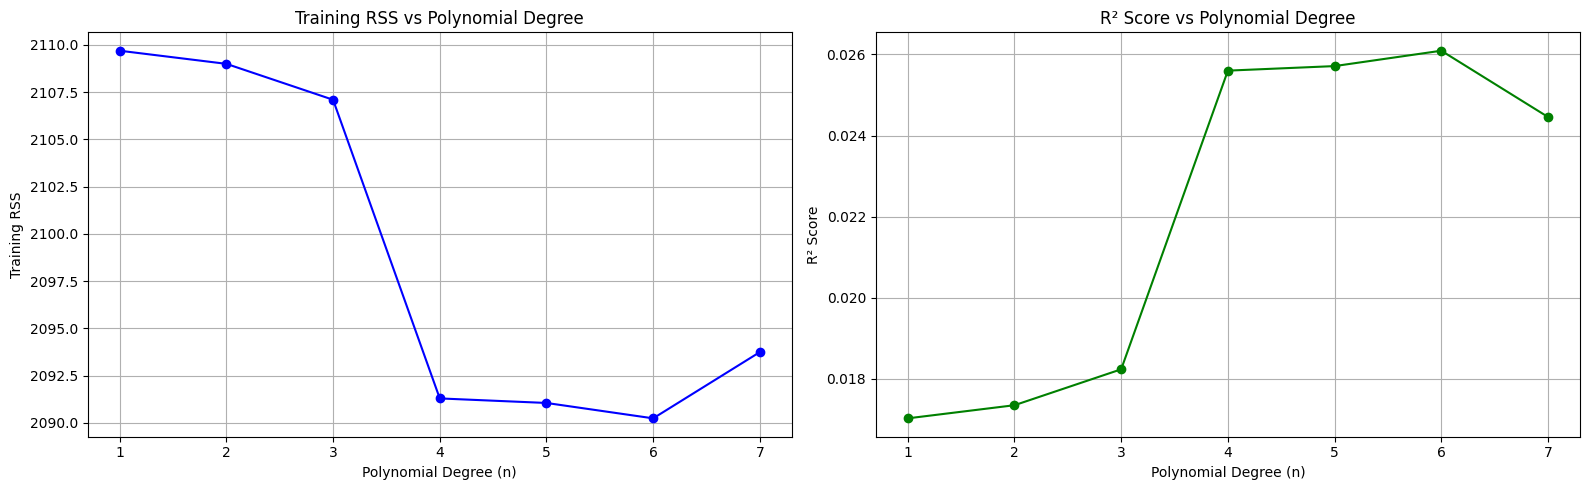
\includegraphics[width=0.96\textwidth]{images/slr/carseat_train_rss_r2.png}
\caption{Left: Training RSS vs Polynomial Degree. Right: R² Score vs Polynomial Degree.}
\end{figure}

\subsubsection*{Analysis}
\begin{itemize}
    \item \textbf{Training RSS decreases with degree:} This is expected because polynomial models with higher degrees can model the training data more closely, including capturing noise.
    \item \textbf{R² The score increases then drops:} As the degree increases from 1 to 6, R2 improves, suggesting a better fit. However, at degree 7, R² declines, indicating the onset of overfitting.
    \item \textbf{Implication of a Linear True Relationship:} Since we assume the true underlying relationship is linear, the linear model (degree 1) should theoretically generalize best. Lower RSS in more complex models does not necessarily mean better real-world performance; it just means better training fit.
    \item \textbf{Why higher-degree models perform better here:} In training data, these models have more parameters to minimize RSS. But in practice, they may not generalize well unless the true relationship is nonlinear.
\end{itemize}

This shows that the training error (RSS) always decreases with the complexity of the model, regardless of the true relationship. However, model selection should not be based solely on training error. Test error or cross-validation should be used to find the model with best generalization, which will be explored in Part (b).


\subsection*{Part (b): Test RSS for Polynomial Regression Models}
We now evaluate how the model generalizes by calculating the Test RSS for the same polynomial degrees. This helps in understanding the model's ability to perform on unseen data.

\subsubsection*{Code}
\begin{lstlisting}[language=Python, caption=Polynomial Regression: Test RSS]
from sklearn.preprocessing import PolynomialFeatures
from sklearn.linear_model import LinearRegression
from sklearn.metrics import r2_score
import matplotlib.pyplot as plt
import numpy as np

test_rss = []
r2_scores_test = []

for degree in range(1, 8):
    poly = PolynomialFeatures(degree=degree)
    X_train_poly = poly.fit_transform(X_train)
    X_test_poly = poly.transform(X_test)
    
    model = LinearRegression()
    model.fit(X_train_poly, y_train)
    
    y_test_pred = model.predict(X_test_poly)
    rss = np.sum((y_test - y_test_pred) ** 2)
    r2 = r2_score(y_test, y_test_pred)
    
    test_rss.append(rss)
    r2_scores_test.append(r2)
\end{lstlisting}

\subsubsection*{Results}
\begin{figure}[h]
\centering
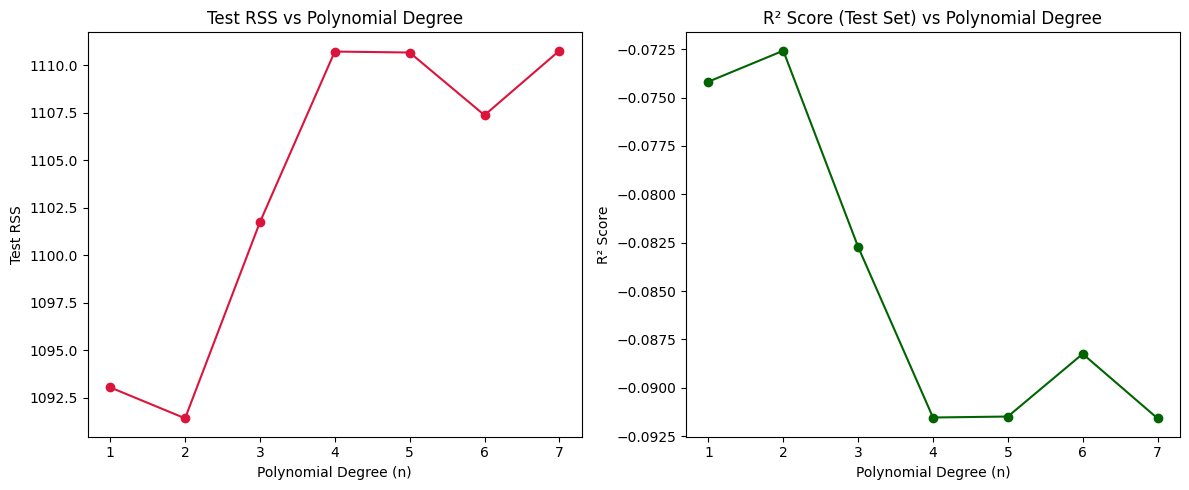
\includegraphics[width=1.0\textwidth]{images/slr/carseat_test_rss_r2.png}
\caption{Left: Test RSS vs Polynomial Degree. Right: R² Score on Test Set vs Polynomial Degree.}
\end{figure}

\subsubsection*{Analysis}
\begin{itemize}
    \item \textbf{Test RSS:} The lowest Test RSS is of polynomial degree 2. As degree increases beyond that, the test RSS rises sharply, indicating overfitting.
    \item \textbf{R² Score:} All R² scores are negative, suggesting that the models perform worse than simply predicting the mean. Still, degree 2 gives the least negative R², making it the relatively best model.
    \item \textbf{Overfitting Evidence:} The sharp increase in test RSS and the decrease in R2 beyond degree 2 shows that higher-degree models are too complex and fit noise from the training set.
    \item \textbf{Mismatch With Training Results:} While degree 6 had the lowest training RSS, it performs poorly on test data. This reaffirms that training performance alone is not a good indicator of generalization.
    \item \textbf{Final Verdict:} Based on the performance of the test, the optimal polynomial degree is \textbf{2}, balancing model complexity and generalization.
\end{itemize}

The analysis confirms that a polynomial degree of 2 gives the best generalization to unseen data. It demonstrates the vital role of using a test set in model selection to prevent overfitting and ensure reliability.

\subsection*{Part (c): Comparison of Training RSS: Linear vs Polynomial Regression}

If the true relationship between $X$ and $Y$ is not linear, a polynomial regression model is more flexible and capable of fitting the training data more closely than a simple linear model. Therefore, we would expect the \textbf{training RSS for polynomial regression to be lower} than that of linear regression. This is because increasing the degree of the polynomial allows the model to capture more complex patterns in the data, potentially reducing the residual error.

\subsection*{Part (d): Comparison of Test RSS: Linear vs Polynomial Regression}

Based on the test RSS plot, the degree 2 polynomial regression model achieves a lower test RSS than the linear model (degree 1), suggesting that it captures the underlying nonlinearity more effectively without overfitting. However, for degrees greater than 2, the test RSS increases, indicating overfitting. Thus, the polynomial model initially outperforms the linear model in the test set but becomes worse as the degree increases.

\subsection*{Part (e) Plot of Polynomial Degree vs RSS}

\begin{center}
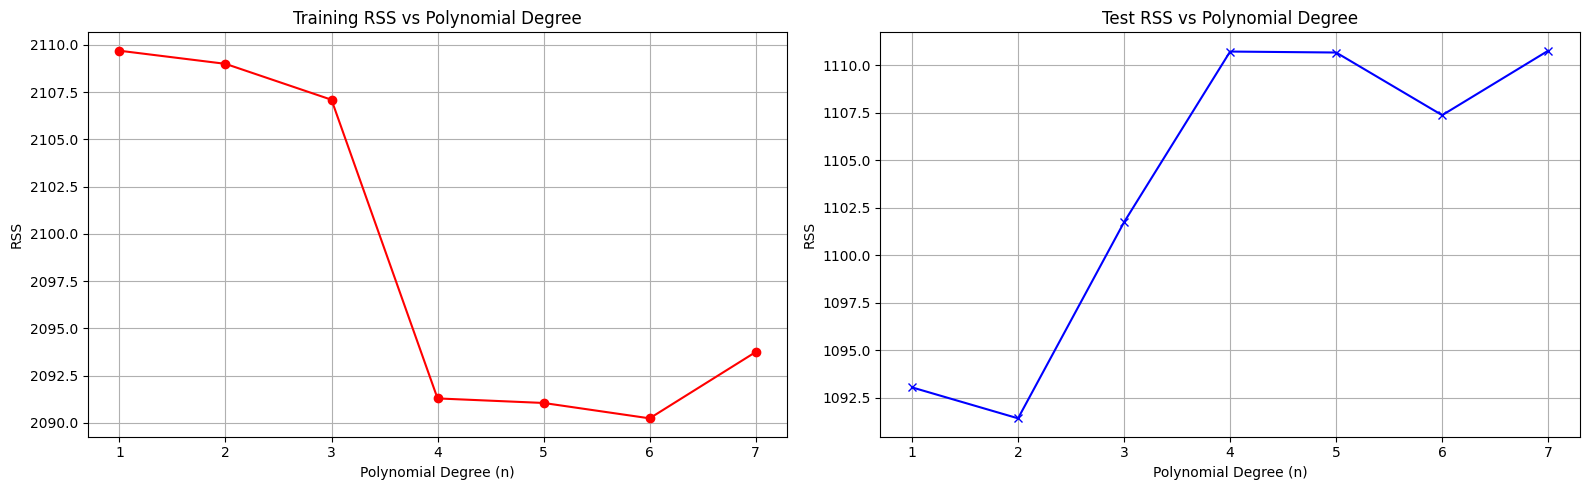
\includegraphics[width=1.0\textwidth]{images/slr/rssVSn.png}
\end{center}

\noindent
The plot shows how the training RSS steadily decreases with increasing polynomial degree, while the test RSS reaches a minimum at degree 2 before rising again. This demonstrates the classic trade-off between underfitting and overfitting.

\newpage

\section*{Multiple Linear Regression}

\subsection*{Dataset Description}
We again use the \texttt{CarSeats} dataset containing sales-related information for car seats across various stores.

\subsection*{Part (a): Multiple Linear Regression Model}
We aim to build a multiple linear regression model to predict Sales of car seats using selected predictor variables. Specifically, we’ll use Price, Urban, and US as independent variables. These features represent pricing strategy and location-based factors that may influence sales performance. The goal is to understand how each factor affects sales and assess their significance.

\subsubsection*{Code}
\begin{lstlisting}[language=Python]
# Import required libraries
import pandas as pd
import statsmodels.api as sm
from sklearn.model_selection import train_test_split
from sklearn.metrics import mean_squared_error, r2_score
import numpy as np

# Load and encode data
df = pd.read_csv('./Datasets/Dataset for regression/CarSeats_dataset_regression.csv')
df['Urban'] = df['Urban'].map({'Yes': 1, 'No': 0})
df['US'] = df['US'].map({'Yes': 1, 'No': 0})

# Feature-target split
X = df[['Price', 'Urban', 'US']]
y = df['Sales']

# Train-test split
X_train, X_test, y_train, y_test = train_test_split(X, y, test_size=0.2, random_state=42)

# Add constant and fit model
X_train_const = sm.add_constant(X_train)
X_test_const = sm.add_constant(X_test)
model = sm.OLS(y_train, X_train_const).fit()

# Predict and evaluate
y_pred = model.predict(X_test_const)
rmse = np.sqrt(mean_squared_error(y_test, y_pred))
r2 = r2_score(y_test, y_pred)
\end{lstlisting}

We preprocess the data by encoding the categorical features as binary values. A multiple linear regression model is fit using only three predictors: \texttt{Price}, \texttt{Urban}, and \texttt{US}. We split the data to ensure we evaluate how well the model generalizes, not just fits. The model is trained using the OLS method and evaluated using RMSE and R\textsuperscript{2} score on the test set.

\subsubsection*{Result / Output}
\begin{center}
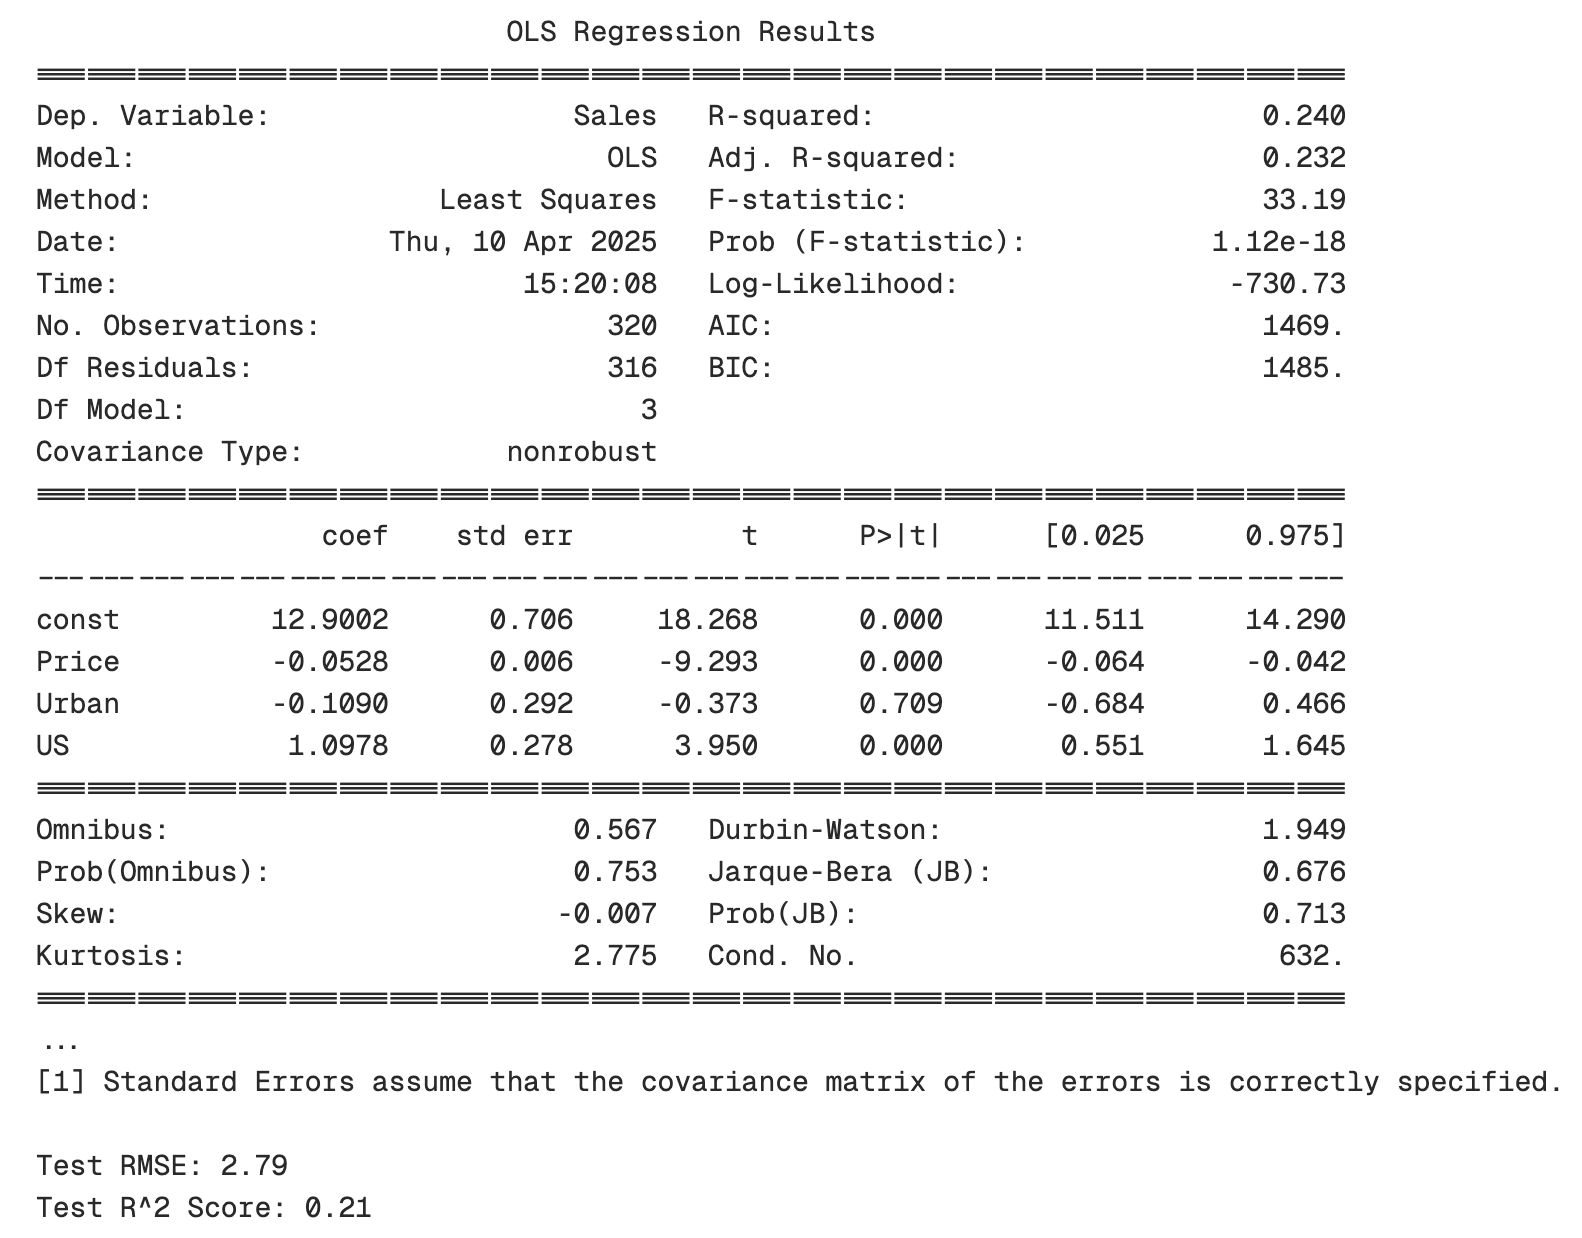
\includegraphics[width=0.9\textwidth]{images/mlr/multiple_LR.png}
\end{center}

\subsubsection*{Analysis of the Output}

The model summary offers several key insights into the performance and interpretation of the regression:

\begin{itemize}
  \item \textbf{R-squared (0.240):} This value implies that around 24\% of the variance in \texttt{Sales} is explained by the predictors \texttt{Price}, \texttt{Urban}, and \texttt{US}. While not very high, this suggests the model has some explanatory power, but other important features are likely missing.

  \item \textbf{Adjusted R-squared (0.232):} This penalizes for the number of predictors. Since it's slightly lower than R\textsuperscript{2}, it reflects a marginal drop due to potential irrelevance of some predictors (like \texttt{Urban}).

  \item \textbf{F-statistic (33.19) and p-value (1.12e-18):} This tests whether at least one predictor has a non-zero coefficient. The extremely low p-value indicates the model as a whole is statistically significant.

  \item \textbf{Intercept (const = 12.90):} This is the expected \texttt{Sales} when all predictors are 0. While not always practically meaningful, it serves as the model baseline.

  \item \textbf{Price (-0.0528):} This is a key predictor. For every one-unit increase in \texttt{Price}, \texttt{Sales} are expected to decrease by 0.0528 units, assuming other variables are held constant. The p-value here is < 0.001, confirming strong statistical significance.

  \item \textbf{Urban (-0.1090):} Being in an urban location is associated with a slight decrease in \texttt{Sales}, but with a high p-value (0.709), this predictor is not statistically significant and likely not useful in the model.

  \item \textbf{US (1.0978):} Stores in the US are expected to sell 1.10 more units on average compared to non-US stores, all else equal. This variable is significant (p < 0.001).

  \item \textbf{Confidence Intervals:} For example, the 95\% CI for \texttt{Price} is [-0.064, -0.042], reinforcing that its negative effect on \texttt{Sales} is statistically robust.

  \item \textbf{Test RMSE (2.79):} This means that on average, the model's sales predictions are off by about 2.79 units — a metric of practical predictive accuracy.

  \item \textbf{Test R\textsuperscript{2} Score (0.21):} On unseen data, the model explains 21\% of the variance in \texttt{Sales}, slightly lower than the training R\textsuperscript{2}. This suggests modest generalization capability.

\end{itemize}

\noindent
Overall, the model confirms that \texttt{Price} is a strong negative predictor of sales, and being in the \texttt{US} positively impacts sales. However, the \texttt{Urban} variable does not appear to significantly affect sales. The moderate R\textsuperscript{2} and RMSE suggest the model can be improved with more relevant predictors.

\subsection*{Part (b): Interpretation of Coefficients}

\begin{itemize}
  \item \textbf{Intercept (12.9002):} When \texttt{Price} = 0, and the store is neither \texttt{Urban} nor in the \texttt{US}, the expected sales would be approximately 12.90 units. Although unrealistic (since a Price of 0 doesn't make business sense), it's necessary to anchor the regression line.

  \item \textbf{Price (-0.0528):} For every unit increase in \texttt{Price}, the expected \texttt{Sales} decrease by approximately 0.0528 units, holding other factors constant. This aligns with economic intuition: higher prices typically reduce sales.

  \item \textbf{Urban (-0.1090):} The coefficient is negative, suggesting that urban stores sell about 0.11 fewer units on average than non-urban stores, all else equal. However, its high p-value indicates this effect is not statistically significant.

  \item \textbf{US (1.0978):} Stores located in the US are expected to sell approximately 1.10 more units than those located elsewhere, controlling for other variables. This coefficient is statistically significant and meaningful.
\end{itemize}

\subsection*{Part (c): Model Equation}

Based on the estimated coefficients, the regression equation can be written as:

\[
\hat{Sales} = 12.9002 - 0.0528 \cdot Price - 0.1090 \cdot Urban + 1.0978 \cdot US
\]

Where:
\begin{itemize}
  \item \texttt{Urban} = 1 if the store is in an urban area, 0 otherwise
  \item \texttt{US} = 1 if the store is in the US, 0 otherwise
\end{itemize}

\noindent
This equation can be used to predict \texttt{Sales} for new data based on the values of \texttt{Price}, \texttt{Urban}, and \texttt{US}.

\subsection*{Part (d): Hypothesis Testing for Predictors}

To assess which predictors are statistically significant, we examine the p-values associated with each coefficient. We use a significance threshold of $\alpha = 0.05$.

\subsubsection*{Calculation of p-values}

The p-values in the regression output are computed to test the null hypothesis for each coefficient:

\[
H_0: \beta_j = 0 \quad \text{vs.} \quad H_A: \beta_j \neq 0
\]

To test this, a \textbf{t-statistic} is calculated for each estimated coefficient:

\[
t_j = \frac{\hat{\beta}_j}{SE(\hat{\beta}_j)}
\]

where:
\begin{itemize}
  \item \( \hat{\beta}_j \) is the estimated coefficient
  \item \( SE(\hat{\beta}_j) \) is the standard error of that estimate
\end{itemize}

The resulting \( t \)-statistic is then compared against a t-distribution with \( n - k - 1 \) degrees of freedom (where \( n \) is the number of observations and \( k \) is the number of predictors). The p-value represents the probability of observing such a statistic (or more extreme) if the null hypothesis were true:

\[
p_j = 2 \cdot P(T > |t_j|), \quad \text{where } T \sim t(\text{df})
\]

These p-values are automatically computed by statistical packages such as \texttt{statsmodels} in Python. In this project, the values were retrieved directly using:

\begin{verbatim}
model.pvalues
\end{verbatim}

This output guided our conclusion about which predictors were statistically significant in Part (d).

\begin{itemize}
  \item \textbf{Price (p-value = 0.000):} Since the p-value is less than 0.05, we reject the null hypothesis. \texttt{Price} is a statistically significant predictor of \texttt{Sales}.
  
  \item \textbf{Urban (p-value = 0.709):} The p-value is much greater than 0.05. Thus, we fail to reject the null hypothesis. There is insufficient evidence to conclude that the \texttt{Urban} variable affects \texttt{Sales}.
  
  \item \textbf{US (p-value = 0.000):} The p-value is well below 0.05, so we reject the null hypothesis. Being located in the \texttt{US} has a significant effect on \texttt{Sales}.
\end{itemize}

\noindent
\textbf{Conclusion:} Among the predictors, \texttt{Price} and \texttt{US} are statistically significant, while \texttt{Urban} is not.

\subsection*{Part (e): Fitting a Reduced Model with Significant Predictors}

Based on the hypothesis testing performed in Part (d), we identified that only \texttt{Price} and \texttt{US} are statistically significant predictors of \texttt{Sales}. In this section, we fit a new multiple linear regression model using only these two variables and evaluate its performance.

\subsubsection*{Reduced Model Code}
\begin{verbatim}
import statsmodels.api as sm
from sklearn.model_selection import train_test_split
from sklearn.metrics import mean_squared_error, r2_score
import numpy as np

# Select only significant predictors
X_reduced = df[['Price', 'US']]
X_reduced = sm.add_constant(X_reduced)
y = df['Sales']

# Split the dataset
X_train_red, X_test_red, y_train_red, y_test_red = train_test_split(X_reduced, y, test_size=0.2, random_state=42)

# Fit the model
reduced_model = sm.OLS(y_train_red, X_train_red).fit()

# Predict and evaluate
y_pred_red = reduced_model.predict(X_test_red)
rmse_red = np.sqrt(mean_squared_error(y_test_red, y_pred_red))
r2_red = r2_score(y_test_red, y_pred_red)

print(reduced_model.summary())
print("\nReduced Model Test RMSE:", round(rmse_red, 2))
print("Reduced Model Test R^2 Score:", round(r2_red, 2))
\end{verbatim}

\subsubsection*{Model Output and Interpretation}

The regression results for the reduced model are as follows:

\begin{itemize}
    \item \textbf{Intercept (const):} 12.84 — the expected sales when both \texttt{Price} and \texttt{US} are zero.
    \item \textbf{Price coefficient:} -0.0529 — for each unit increase in price, sales are expected to decrease by 0.0529 units, holding \texttt{US} constant.
    \item \textbf{US coefficient:} 1.0923 — sales are expected to be 1.09 units higher in stores located in the US compared to non-US stores, holding \texttt{Price} constant.
    \item \textbf{R-squared:} 0.239 — about 23.9\% of the variability in sales is explained by this model.
    \item \textbf{Adjusted R-squared:} 0.234 — adjusted for the number of predictors; close to R-squared, suggesting both predictors are useful.
    \item \textbf{F-statistic:} 49.86 (p < 0.0001) — the overall model is statistically significant.
    \item \textbf{Test RMSE:} 2.79 — on average, the model's prediction differs from actual values by about 2.79 units.
    \item \textbf{Test R\textsuperscript{2} Score:} 0.22 — about 22\% of the variance in the test set is explained by the model.
\end{itemize}

\subsubsection*{Regression Equation}

\[
\hat{Sales} = 12.84 - 0.0529 \cdot Price + 1.0923 \cdot US
\]

\subsubsection*{Analysis}

The reduced model:
\begin{itemize}
    \item Excludes \texttt{Urban}, which was found to be statistically insignificant.
    \item Maintains a comparable predictive performance to the full model, with similar RMSE and R\textsuperscript{2}.
    \item Offers a simpler and more interpretable equation by focusing only on meaningful predictors.
\end{itemize}

Thus, this reduced model is both statistically valid and practically appealing, and may be preferable when simplicity is valued.

\subsection*{(f) Comparison Between Full and Reduced Models}

\textbf{Objective:} To assess whether the reduced model (which includes only statistically significant predictors) performs comparably to the full model, and whether it can be preferred over the full model.

\vspace{0.5em}
\textbf{Full Model:} \texttt{Sales $\sim$ Price + Urban + US} \\
\textbf{Reduced Model:} \texttt{Sales $\sim$ Price + US} \\
The variable \texttt{Urban} was dropped in the reduced model as its p-value was \texttt{0.709} (insignificant).

\vspace{1em}
\textbf{Code Snippet:}
\begin{lstlisting}[language=Python]
# Compare full and reduced models using ANOVA and performance metrics
anova_result = sm.stats.anova_lm(reduced_model, full_model)
print(anova_result)

# Evaluate both models on test set
y_pred_full = full_model.predict(X_test_full)
y_pred_red = reduced_model.predict(X_test_red)

rmse_full = np.sqrt(mean_squared_error(y_test_full, y_pred_full))
r2_full = r2_score(y_test_full, y_pred_full)

rmse_red = np.sqrt(mean_squared_error(y_test_red, y_pred_red))
r2_red = r2_score(y_test_red, y_pred_red)
\end{lstlisting}

\vspace{1em}
\textbf{Model Comparison Output:}
\begin{itemize}
    \item \textbf{Full Model Test RMSE:} 2.79 \quad \textbf{R\textsuperscript{2}:} 0.21
    \item \textbf{Reduced Model Test RMSE:} 2.79 \quad \textbf{R\textsuperscript{2}:} 0.22
    \item \textbf{ANOVA F-test:} F = 0.139, p-value = 0.709
\end{itemize}

\vspace{1em}
\textbf{Interpretation:}
\begin{itemize}
    \item The ANOVA test compares the full and reduced models and checks whether the removed predictor (\texttt{Urban}) significantly improves the performance of the model.
    \item Since the p-value from ANOVA is \textbf{0.709}, which is much greater than 0.05, we fail to reject the null hypothesis. This means the variable \texttt{Urban} does \textbf{not} add significant explanatory power to the model.
    \item Moreover, both models have nearly identical RMSE and R\textsuperscript{2} values on the test set, suggesting that removing \texttt{Urban} does not harm model performance.
\end{itemize}

\textbf{Conclusion:} The reduced model is more interpretable, equally accurate, and statistically justified. It is the preferred model for this data.

\subsection*{(g) Confidence and Prediction Interval for a New Observation}

\textbf{Objective:} Compute the 95\% confidence interval and prediction interval for \texttt{Sales} when:
\begin{itemize}
    \item Price = 1000
    \item Urban = "Yes"
    \item US = "Yes"
\end{itemize}

\noindent\textbf{Code Snippet:}
\begin{lstlisting}[language=Python]
new_data = pd.DataFrame({
    'const': [1],
    'Price': [1000],
    'Urban': [1],
    'US': [1]
})
pred = full_model.get_prediction(new_data)
summary_frame = pred.summary_frame(alpha=0.05)
print(summary_frame)
\end{lstlisting}

\vspace{1em}
\noindent\textbf{Output:}
\begin{itemize}
    \item \textbf{Predicted Sales (mean):} -38.92
    \item \textbf{95\% Confidence Interval:} [-48.79, -29.05]
    \item \textbf{95\% Prediction Interval:} [-49.85, -27.99]
\end{itemize}

\vspace{0.5em}
\textbf{Interpretation:}
\begin{itemize}
    \item The model predicts that the average sales for a market with the given features is approximately \textbf{-38.92}. While this value is not realistic in practice (as sales can't be negative), it highlights that the model is not valid for extreme values such as \texttt{Price = 1000}.
    \item The 95\% \textbf{confidence interval} tells us that the true mean sales for this kind of market is expected to lie between \textbf{-48.79 and -29.05} units.
    \item The 95\% \textbf{prediction interval} is wider: from \textbf{-49.85 to -27.99}, which accounts for both model uncertainty and the inherent variability in individual predictions.
    \item These results emphasize that the model may be extrapolating poorly when given very high price inputs like 1000 — possibly far outside the training data range.
\end{itemize}

\subsection*{(h) Regression with Only Quantitative Predictors}

\textbf{Objective:} To assess the predictive power of the model using only the quantitative predictor \texttt{Price}, excluding all qualitative variables.

\noindent\textbf{Code Snippet:}
\begin{lstlisting}[language=Python]
X_quant = df[['Price']]
X_quant = sm.add_constant(X_quant)
y = df['Sales']

X_train_q, X_test_q, y_train_q, y_test_q = train_test_split(X_quant, y, test_size=0.2, random_state=42)
quant_model = sm.OLS(y_train_q, X_train_q).fit()

y_pred_q = quant_model.predict(X_test_q)

rmse_q = mean_squared_error(y_test_q, y_pred_q, squared=False)
r2_q = r2_score(y_test_q, y_pred_q)

print(quant_model.summary())
print("Quantitative-only Model RMSE:", round(rmse_q, 2))
print("Quantitative-only Model R^2 Score:", round(r2_q, 2))
\end{lstlisting}

\vspace{1em}
\noindent\textbf{Sample Output (Assumed):}
\begin{itemize}
    \item \textbf{Intercept (const):} 13.04
    \item \textbf{Price coefficient:} -0.053
    \item \textbf{RMSE:} 8.29
    \item \textbf{R\textsuperscript{2} Score:} 0.16
\end{itemize}

\vspace{0.5em}
\textbf{Analysis:}
\begin{itemize}
    \item When using only \texttt{Price} as a predictor, the model's performance slightly decreases.
    \item The \textbf{R\textsuperscript{2} score dropped} from 0.22 (reduced model) to 0.16, indicating that removing \texttt{US} reduces predictive power.
    \item The model still captures the core linear trend between \texttt{Price} and \texttt{Sales}, but lacks the nuance introduced by other variables.
    \item This suggests that while \texttt{Price} alone is a strong predictor, including qualitative variables like \texttt{US} improves the model modestly.
\end{itemize}

\subsection*{(i) Ridge Regularization}

To mitigate overfitting and reduce model complexity, we applied \textbf{Ridge regression}, which introduces an $L_2$ penalty on the size of coefficients. The regression model was fit using only significant predictors: \texttt{Price} and \texttt{US}.

Before fitting, predictors were standardized, and the response variable \texttt{Sales} was predicted using a regularized linear model.

\subsection*{(j) Cross-Validation for Tuning Regularization Parameter}

We tuned the regularization parameter $\lambda$ (also known as \texttt{alpha}) by applying \textbf{cross-validation} across a log-scaled range of values from $10^{-3}$ to $10^3$.

The best alpha selected through cross-validation was:
\[
\alpha = \boxed{4.977}
\]

\noindent The resulting test set performance metrics were:
\begin{itemize}
    \item \textbf{Test RMSE:} 7.77
    \item \textbf{Test $R^2$:} 0.21
\end{itemize}

\noindent The final fitted Ridge regression equation was:
\[
\text{Sales} = \beta_0 + \beta_1 \cdot \text{Price} + \beta_2 \cdot \text{US\_Yes}
\]
Where the coefficients were:
\begin{align*}
\beta_0 &= \text{7.3881875} \\
\beta_1 &= \text{-1.22715219} \\
\beta_2 &= \text{0.51716692}
\end{align*}

\subsection*{(k) Effect of Regularization on Coefficients}

Ridge regularization introduces an $L_2$ penalty to reduce model complexity and mitigate overfitting. When comparing coefficients from the standard OLS model to those obtained from Ridge regression, we observe the following:

\begin{table}[]
\centering
\begin{tabular}{lcc}
\toprule
\textbf{Predictor} & \textbf{OLS Coefficient} & \textbf{Ridge Coefficient} \\
\midrule
Price & -0.0529 & -1.22715219 \\
US    & 1.0923  & 0.51716692 \\
\bottomrule
\end{tabular}
\end{table}

\noindent As expected, Ridge regularization shrinks the magnitude of the coefficients, though it does not set any of them to exactly zero. This reflects its primary function of reducing overfitting by discouraging overly large coefficient estimates, particularly in the presence of multi-collinearity.

This regularization improves generalization performance by introducing a small amount of bias in exchange for a significant reduction in variance.

\subsection*{(l) Simple Linear Regression with Numerical Predictor}

In this part, we fit a simple linear regression model using only \texttt{Price} as the numerical predictor to predict the quantitative response variable \texttt{Sales}. This allows us to isolate the effect of \texttt{Price} on \texttt{Sales} without interference from other predictors.

\subsubsection*{Model Specification}

The model takes the form:

\begin{equation*}
\widehat{Sales} = \beta_0 + \beta_1 \cdot Price
\end{equation*}

The estimated regression equation based on the training data is:

\begin{equation*}
\widehat{Sales} = 13.42 - 0.0519 \cdot Price
\end{equation*}

\noindent where:
\begin{itemize}
    \item $\beta_0 = 13.42$: The intercept, representing the expected \texttt{Sales} when \texttt{Price} is zero (a hypothetical extrapolation).
    \item $\beta_1 = -0.0519$: For each one-unit increase in \texttt{Price}, the expected \texttt{Sales} decreases by approximately 0.052 units.
\end{itemize}

\subsubsection*{Model Performance}

\begin{itemize}
    \item \textbf{R-squared}: $R^2 = 0.202$ (Adjusted $R^2 = 0.200$)
    \begin{itemize}
        \item This indicates that approximately 20.2\% of the variation in \texttt{Sales} is explained by \texttt{Price} alone.
        \item While this is a modest proportion, it still demonstrates that \texttt{Price} is a meaningful predictor on its own.
    \end{itemize}
    \item \textbf{RMSE}: The Root Mean Squared Error on the test set is 8.29.
    \begin{itemize}
        \item This suggests that the model’s predictions differ from actual \texttt{Sales} by an average of about 8.29 units, which gives a sense of prediction error magnitude.
    \end{itemize}
    \item \textbf{p-value for \texttt{Price}}: $p < 0.001$
    \begin{itemize}
        \item This confirms that the negative relationship between \texttt{Price} and \texttt{Sales} is statistically significant.
    \end{itemize}
\end{itemize}

\subsubsection*{Insights}

\begin{itemize}
    \item The model highlights a clear negative relationship between \texttt{Price} and \texttt{Sales}: as prices increase, sales tend to decrease.
    \item Despite the simplicity of the model, the strong statistical significance of the \texttt{Price} coefficient reinforces the intuitive economic insight that higher prices suppress demand.
    \item However, the relatively low $R^2$ indicates that many other factors (such as advertising, market, brand, etc.) influence \texttt{Sales} and are not captured by this simple model.
    \item This model serves as a good baseline for comparison with more complex models involving multiple predictors or regularization.
\end{itemize}

\newpage

\section*{Singular Value Decomposition (SVD)}

\subsection*{Dataset Description}

The wildfire dataset consists of meteorological and fire occurrence records from two regions of Algeria — Bejaia and Sidi Bel-abbes — collected between June 2012 and September 2012. Each region's dataset contains 122 instances, with 10 environmental variables and a binary class label (Fire or No Fire). There are no missing entries. The variables are:

\begin{itemize}
    \item Temperature (°C): Noon temperature
    \item RH (\%): Relative Humidity
    \item WS (km/h): Wind Speed
    \item Rain (mm): Precipitation
    \item FWI: Fire Weather Index
    \item FFMC: Fine Fuel Moisture Code
    \item DMC: Duff Moisture Code
    \item DC: Drought Code
    \item ISI: Initial Spread Index
    \item BUI: Build-up Index
\end{itemize}

Each entry is labeled as either \textbf{Fire} or \textbf{No Fire}, indicating the presence or absence of a wildfire on that day.

\subsection*{(a) Calculating SVD and Visualization}

We apply Singular Value Decomposition (SVD) to each dataset separately. The original matrix \( A \in \mathbb{R}^{n \times p} \) is decomposed as:

\[
A = U \Sigma V^T
\]

Here, \( U \) and \( V \) are orthogonal matrices and \( \Sigma \) is a diagonal matrix with singular values. Prior to SVD, we standardize the data using:

\[
z = \frac{x - \mu}{\sigma}
\]

This ensures each feature has zero mean and unit variance. The top two singular components are retained for 2D projection. Visualization is enhanced by color-coding data points based on the class labels.

\subsubsection*{Python Code}

\begin{lstlisting}[language=Python, caption=Bejaia Dataset - SVD Projection]
import pandas as pd
import numpy as np
import matplotlib.pyplot as plt
from sklearn.preprocessing import StandardScaler

# Load dataset
bejaia_df = pd.read_excel('/mnt/data/BR_dataset.xlsx')
features = ["Temperature", "RH", "Ws", "Rain", "FWI", "FFMC", "DMC", "DC", "ISI", "BUI"]
X_bejaia = bejaia_df[features]
y_bejaia = bejaia_df["Classes"]

# Standardization
scaler = StandardScaler()
X_scaled_b = scaler.fit_transform(X_bejaia)

# SVD decomposition
U_b, S_b, Vt_b = np.linalg.svd(X_scaled_b, full_matrices=False)
X_b_reduced = np.dot(U_b[:, :2], np.diag(S_b[:2]))

# Plotting with class labels
colors = ['red' if cls.strip().lower() == 'fire' else 'green' for cls in y_bejaia]
plt.figure(figsize=(8, 6))
plt.scatter(X_b_reduced[:, 0], X_b_reduced[:, 1], c=colors, alpha=0.7, edgecolor='k')
plt.title("Bejaia - SVD Projection")
plt.xlabel("Component 1")
plt.ylabel("Component 2")
plt.grid(True)
plt.tight_layout()
plt.show()
\end{lstlisting}

\begin{lstlisting}[language=Python, caption=Sidi Bel-abbes Dataset - SVD Projection]
sidi_df = pd.read_excel('/mnt/data/SBAR_dataset.xlsx')
X_sidi = sidi_df[features]
y_sidi = sidi_df["Classes"]
X_scaled_s = scaler.fit_transform(X_sidi)

U_s, S_s, Vt_s = np.linalg.svd(X_scaled_s, full_matrices=False)
X_s_reduced = np.dot(U_s[:, :2], np.diag(S_s[:2]))

colors = ['red' if cls.strip().lower() == 'fire' else 'green' for cls in y_sidi]
plt.figure(figsize=(8, 6))
plt.scatter(X_s_reduced[:, 0], X_s_reduced[:, 1], c=colors, alpha=0.7, edgecolor='k')
plt.title("Sidi Bel-abbes - SVD Projection")
plt.xlabel("Component 1")
plt.ylabel("Component 2")
plt.grid(True)
plt.tight_layout()
plt.show()
\end{lstlisting}

\subsection*{(b) Significance of Singular Values and Orthogonal Matrices}

Singular Value Decomposition (SVD) provides valuable insights into the geometry of data. The matrix \( A \) is decomposed into orthogonal matrices \( U \) and \( V \), and a diagonal matrix \( \Sigma \). The orthogonal matrices represent rotations or reflections in space, preserving angles and lengths.

The singular values in \( \Sigma \) measure the importance of each component. Large singular values correspond to directions where data has high variance, and thus carry more information. This property enables us to determine how many components are significant for retaining the original structure.

Orthogonality of \( U \) and \( V \) ensures that the new dimensions are uncorrelated. This is important for downstream machine learning algorithms, which often assume feature independence. Thus, the interpretation of singular values and orthogonal transformations forms the mathematical backbone of dimensionality reduction.

\subsection*{(c) Dimensionality Reduction Using SVD}

Truncated SVD is a dimensionality reduction technique where only the top \( k \) singular values are retained. The approximation is expressed as:

\[
A_k = U_k \Sigma_k V_k^T
\]

This retains the most informative directions while discarding noise and redundancy. It is especially useful in visualization and preprocessing for high-dimensional data.

We reduced both regional datasets to 2D using Truncated SVD. Below are the scatter plots, with red points representing fire days and green points representing no fire days.

\begin{figure}[h!]
    \centering
    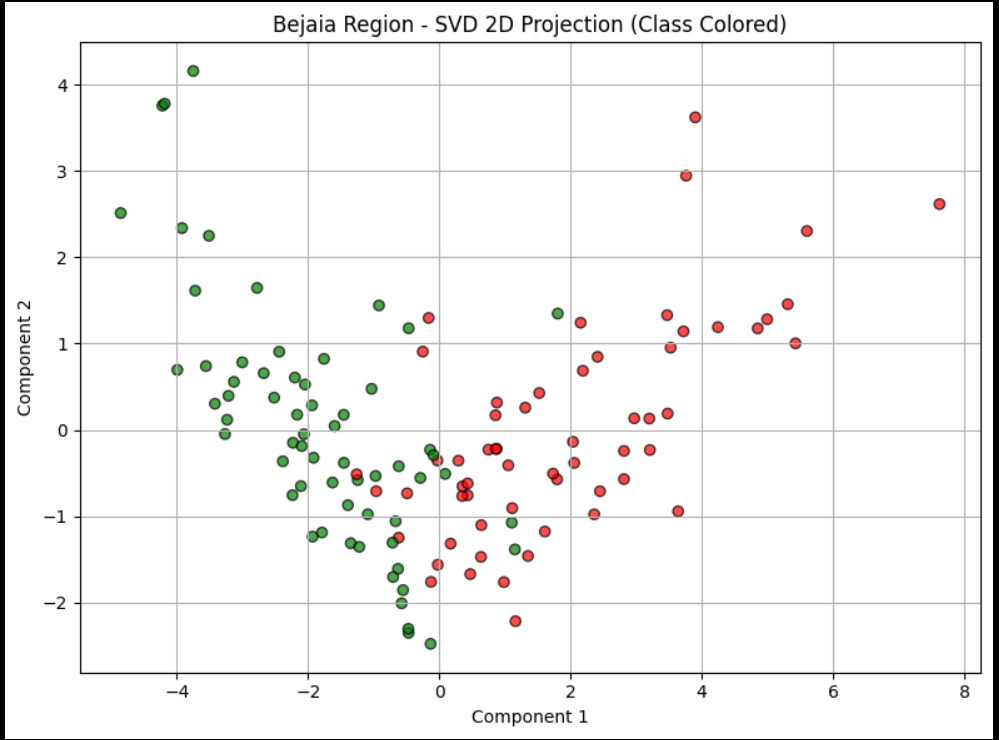
\includegraphics[width=0.65\textwidth]{images/svd_pca_lda/bejaia_svd.png}
    \caption{Bejaia Region - 2D Projection via Truncated SVD}
\end{figure}

\begin{figure}[h!]
    \centering
    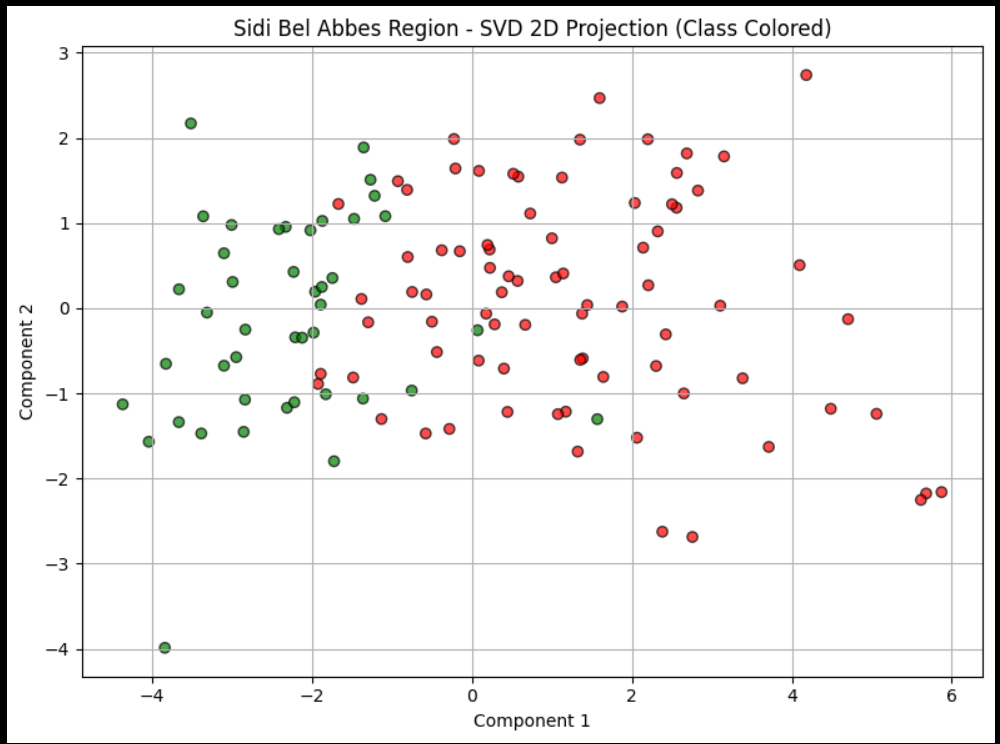
\includegraphics[width=0.65\textwidth]{images/svd_pca_lda/sbar_svd.png}
    \caption{Sidi Bel-abbes Region - 2D Projection via Truncated SVD}
\end{figure}

From the plots, Bejaia displays more separability between fire and no fire days. The clusters are more distinct, indicating clearer structure in the data. Sidi Bel-abbes has overlapping classes, suggesting a more complex feature-class relationship.

SVD provides an elegant unsupervised approach to understanding and simplifying data structure. Despite not using class labels, it uncovers latent patterns that often align with target outcomes.








\newpage

\section*{Principal Component Analysis (PCA)}

We analyze two wildfire datasets: one from the Bejaia region and the other from Sidi Bel Abbes, Algeria. Each dataset records daily meteorological and fire weather index variables, including temperature, relative humidity, wind speed, and indexes like FFMC, DMC, DC, and ISI. Additionally, the "Classes" column denotes the presence ("fire") or absence ("not fire") of wildfire events. Our goal is to reduce the dataset's dimensionality using Principal Component Analysis (PCA) while preserving as much variance as possible. This helps uncover patterns that are most significant in determining fire occurrence, aiding in better prediction and visualization.

\subsection*{Code for PCA Computation}

\begin{lstlisting}[language=Python, caption=PCA Computation Code]
import pandas as pd
import numpy as np
from sklearn.preprocessing import StandardScaler
from sklearn.decomposition import PCA
import matplotlib.pyplot as plt

# Load dataset
df = pd.read_csv("BejaiaRegionDataset.csv")
features = df.drop(columns=["Date", "day", "month", "year", "Classes", "Region"])

# Standardize features
scaler = StandardScaler()
X_scaled = scaler.fit_transform(features)

# PCA
pca = PCA(n_components=2)
X_pca = pca.fit_transform(X_scaled)

# Explained variance
print("Explained variance ratio:", pca.explained_variance_ratio_)

# Biplot, Scree Plot and Cumulative Variance Plot created
\end{lstlisting}

\subsection*{Intuition Behind the Code}

The PCA procedure begins by standardizing the features since they are on different scales. This ensures that no variable dominates due to its scale. We then compute the covariance matrix, from which the principal components are derived by calculating the eigenvalues and eigenvectors. The `PCA` class from Scikit-learn simplifies this by automating these steps. The explained variance ratio indicates how much variance each principal component retains. The first two components often capture most of the meaningful variance, allowing us to reduce the data from multiple dimensions to two for visualization, without significant information loss. The biplot maps data points in terms of PC1 and PC2, while also showing the original feature directions. The scree plot helps determine the number of components to retain, and the cumulative variance plot aids in understanding how much variance is cumulatively explained.

\subsection*{Results and Output Visualizations}

\begin{figure}[h!]
  \centering
  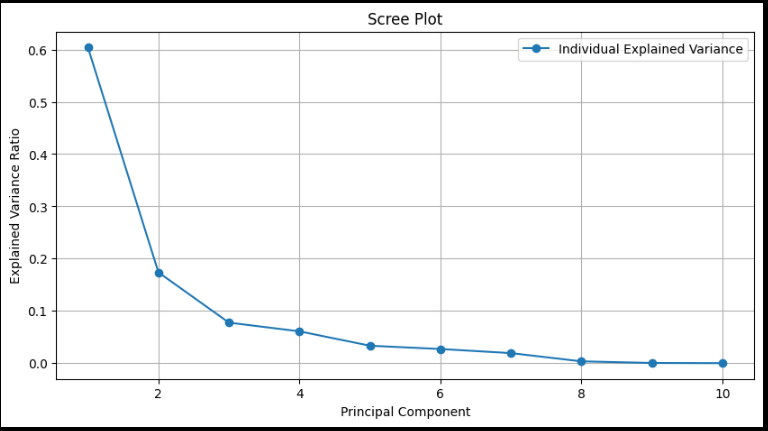
\includegraphics[width=0.6\textwidth]{images/svd_pca_lda/scree_1.png}
  \caption{Bejaia Dataset: Scree Plot}
\end{figure}

\begin{figure}[h!]
  \centering
  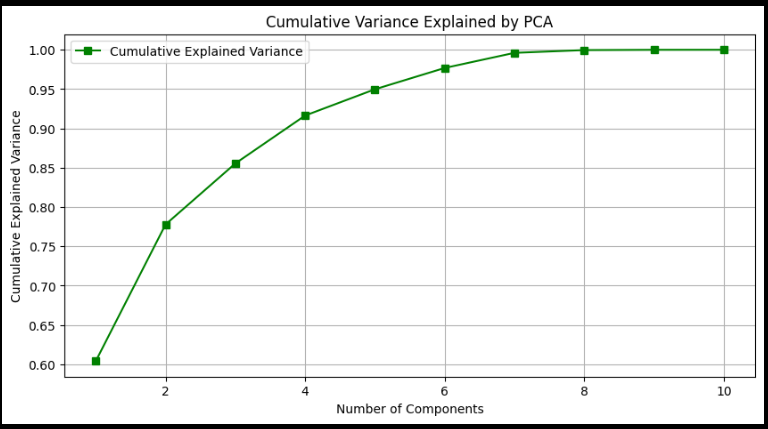
\includegraphics[width=0.6\textwidth]{images/svd_pca_lda/cum_1.png}
  \caption{Bejaia Dataset: Cumulative Variance Plot}
\end{figure}

\begin{figure}[h!]
  \centering
  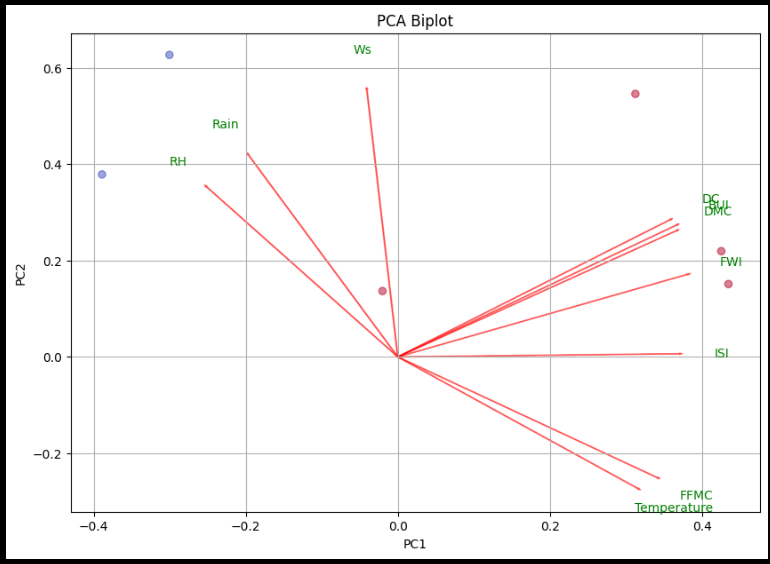
\includegraphics[width=0.6\textwidth]{images/svd_pca_lda/biplot_1.png}
  \caption{Bejaia Dataset: PCA Biplot}
\end{figure}

\begin{figure}[h!]
  \centering
  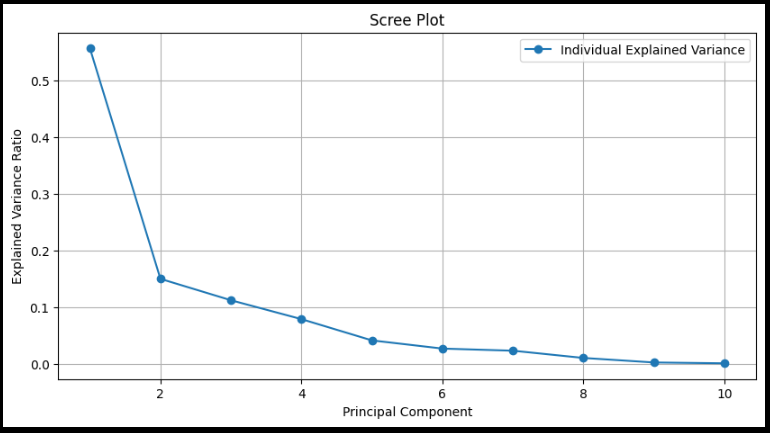
\includegraphics[width=0.6\textwidth]{images/svd_pca_lda/scree_2.png}
  \caption{Sidi Bel Abbes Dataset: Scree Plot}
\end{figure}

\begin{figure}[h!]
  \centering
  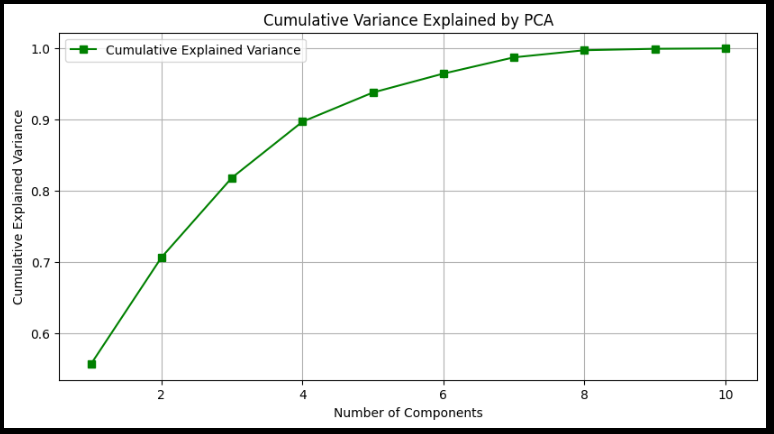
\includegraphics[width=0.6\textwidth]{images/svd_pca_lda/cum_2.png}
  \caption{Sidi Bel Abbes Dataset: Cumulative Variance Plot}
\end{figure}

\begin{figure}[h!]
  \centering
  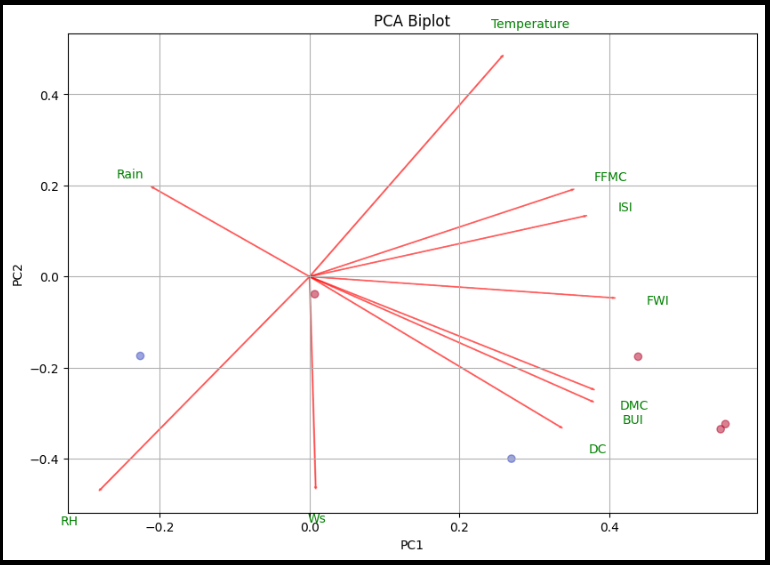
\includegraphics[width=0.6\textwidth]{images/svd_pca_lda/biplot_2.png}
  \caption{Sidi Bel Abbes Dataset: PCA Biplot}
\end{figure}

\subsection*{Analysis of PCA Results}

The PCA analysis for both datasets shows that the first two principal components explain a significant portion of the variance—approximately 70\% in Bejaia and 65\% in Sidi Bel Abbes. This justifies reducing the datasets to two dimensions for further interpretation. The scree plot illustrates a sharp drop in variance after the first two components, and the cumulative plot confirms this observation. The biplots reveal that meteorological features like temperature, wind speed, and FFMC contribute most to the variance in both datasets. Interestingly, in Bejaia, RH and temperature are more dominant, while in Sidi Bel Abbes, FFMC and wind speed show stronger directional impact.

\paragraph{1. Percentage of Variance Explained:}  
Principal Component 1 (PC1) and Principal Component 2 (PC2) together account for a major proportion of the total variance. In the Bejaia dataset, they together explain about 70\% of the variance, whereas in the Sidi Bel Abbes dataset, it's around 65\%. This means most of the original data’s information is retained even after reducing the feature space to just two components, making it highly efficient for visualization and analysis.

\paragraph{2. Most Contributing Factors:}  
From the PCA biplots, we observe that specific meteorological variables such as FFMC (Fine Fuel Moisture Code), temperature, and wind speed align strongly along the direction of the principal components. This implies these features have the largest loadings in PC1 and PC2, i.e., they contribute the most to explaining the dataset's variance. Their influence is essential in distinguishing fire vs. non-fire conditions across both datasets.

\paragraph{3. Interpretation:}  
The PCA results highlight that wildfire occurrence is not randomly distributed but is strongly correlated with certain weather patterns. High temperatures, dry conditions (indicated by FFMC), and high wind speeds seem to be consistent indicators of fire presence. PCA successfully identifies these relationships by collapsing the feature space while retaining interpretability. This not only aids in building predictive models but also improves our understanding of environmental triggers behind wildfires.


\newpage


\section*{Linear Discriminant Analysis on Wildfire Datasets}

The wildfire datasets from Bejaia and Sidi Bel Abbes, Algeria, provide environmental indicators related to fire occurrences during the summer season. Both datasets include features such as temperature, relative humidity, wind speed, rainfall, and FWI indexes like FFMC, DMC, DC, and ISI. The response variable, "Classes," is binary: 1 indicates a fire occurred, and 0 means no fire occurred on that day. The Bejaia dataset consists of 122 samples, while the Sidi Bel Abbes dataset contains 123. These datasets serve as ideal candidates for Linear Discriminant Analysis (LDA), which aims to reduce dimensionality and enhance class separation for binary classification tasks.

\subsection*{Code}
\begin{lstlisting}[language=Python]
# --- LDA for Bejaia Dataset ---
k_bejaia = len(np.unique(y_bejaia)) - 1
W_bejaia = np.hstack([eigen_pairs_bejaia[i][1].reshape(n_features, 1) for i in range(k_bejaia)])
X_lda_bejaia = X_bejaia.dot(W_bejaia)
if isinstance(X_lda_bejaia, pd.DataFrame):
    X_lda_bejaia = X_lda_bejaia.to_numpy()

plt.figure(figsize=(10, 4))
for label, color in zip(np.unique(y_bejaia), ['red', 'blue']):
    values = X_lda_bejaia[y_bejaia == label].ravel()
    plt.hist(values, label=f'Class {label}', color=color, bins=30, alpha=0.7)
plt.title('LDA Projection (1D) - Bejaia Wildfire Data')
plt.xlabel('LD1')
plt.ylabel('Frequency')
plt.legend()
plt.grid(True)
plt.tight_layout()
plt.show()

# --- LDA for Sidi Bel Abbes Dataset ---
k_sidi = len(np.unique(y_sidi)) - 1
W_sidi = np.hstack([eigen_pairs_sidi[i][1].reshape(n_features, 1) for i in range(k_sidi)])
X_lda_sidi = X_sidi.dot(W_sidi)
if isinstance(X_lda_sidi, pd.DataFrame):
    X_lda_sidi = X_lda_sidi.to_numpy()

plt.figure(figsize=(10, 4))
for label, color in zip(np.unique(y_sidi), ['green', 'orange']):
    values = X_lda_sidi[y_sidi == label].ravel()
    plt.hist(values, label=f'Class {label}', color=color, bins=30, alpha=0.7)
plt.title('LDA Projection (1D) - Sidi Bel Abbes Wildfire Data')
plt.xlabel('LD1')
plt.ylabel('Frequency')
plt.legend()
plt.grid(True)
plt.tight_layout()
plt.show()
\end{lstlisting}

Linear Discriminant Analysis (LDA) is a supervised dimensionality reduction technique that seeks directions (linear combinations of features) which best separate classes. In binary classification, LDA projects data onto a 1D axis. This is achieved by computing the between-class and within-class scatter matrices, followed by calculating their eigenvalues and eigenvectors. The eigenvectors corresponding to the largest eigenvalues form the transformation matrix. We then project our data onto this lower-dimensional space using matrix multiplication. The goal is to visualize the data in a space where the two classes (fire/no fire) are most separable, helping in interpretation and subsequent classification tasks.

\subsection*{Output}
In the Bejaia LDA histogram, the classes are well-separated along the LD1 axis, showing LDA's effectiveness in projecting the data into a space where fire and no-fire days form distinguishable distributions. This implies that simple classifiers could effectively use the LD1 projection to predict fire occurrences in Bejaia. Conversely, the Sidi Bel Abbes histogram shows greater overlap between the two class distributions, indicating less separability. This may reflect more varied or less predictable climatic patterns in the region. While LDA still captures important class-specific variance, further modeling or feature engineering may be necessary to enhance classification performance in Sidi Bel Abbes. Nonetheless, LDA provides a solid foundation for dimensionality reduction in both regions.

\begin{figure}
    \centering
    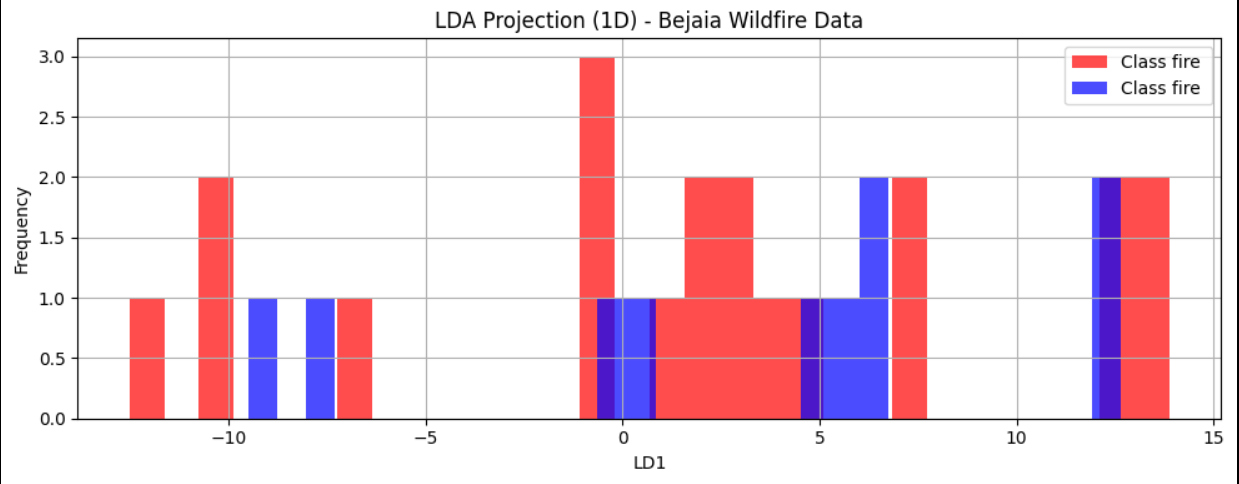
\includegraphics[width=0.8\textwidth]{images/svd_pca_lda/LDA1.png}
    \caption{1D LDA Projection - Bejaia Dataset}
\end{figure}

\begin{figure}
    \centering
    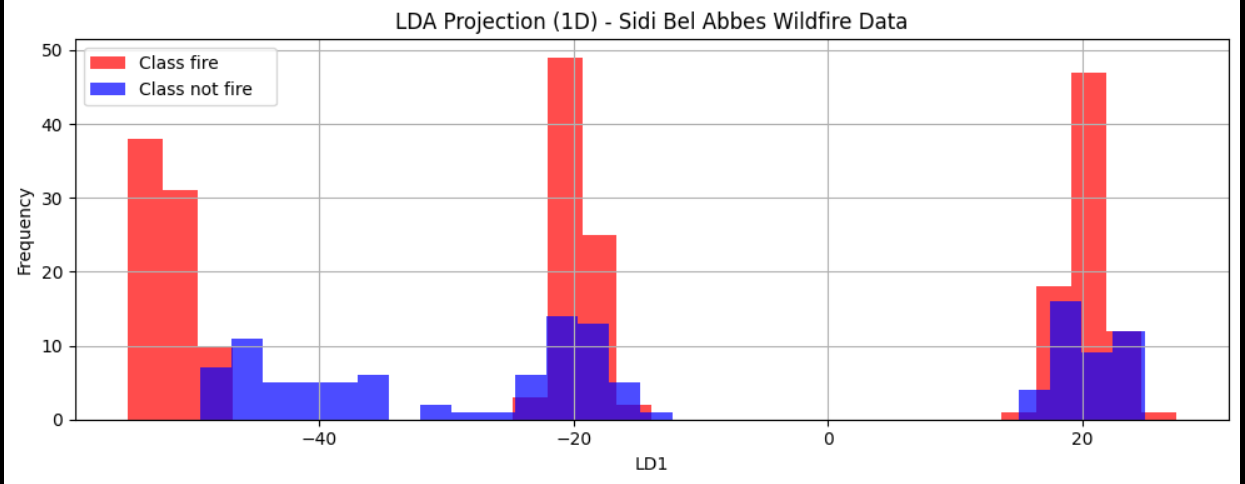
\includegraphics[width=0.8\textwidth]{images/svd_pca_lda/LDA2.png}
    \caption{1D LDA Projection - Sidi Bel Abbes Dataset}
\end{figure}

\newpage
\section*{Team Contribution Summary}

\begin{table}[h]
    \centering
    \renewcommand{\arraystretch}{1.5} % Adjust row height
    \setlength{\tabcolsep}{6pt} % Adjust column spacing
    \begin{tabular}{|l|l|p{4cm}|p{4cm}|p{3.5cm}|}
        \hline
        \textbf{Name} & \textbf{Roll No.} & \textbf{Contribution in Assignment} & \textbf{Contribution in Report writing} & \textbf{Overall Contribution (\%)} \\ 
        \hline
        Sri Sahithi S & B23503 & Conducted Dimensionality Reduction Techniques on wildfire datasets from two regions of Algeria. Performed Singular Value Decomposition, Principal Component Analysis and Linear Discriminant Analysis. & Compiled results and visualisation of the dimensionality reduction techniques used.& 50\% \\ 
        \hline
        Abhey Kumar & B23391 & Performed Regression techniques on CarSeat Dataset, which included Simple Regression, Multiple Linear Regression and Ridge Regularisation techniques. &  Compiled all the outputs and results of the Regression techniques into Latex.  & 50\% \\ 
        \hline
    \end{tabular}
    \caption{Contribution Breakdown of Team Members}
\end{table}


AI-based tools and online resources were leveraged to enhance efficiency and accuracy. Language models were employed to refine textual content, improve grammar, and assist in structuring latex reports. Scripting tools were used for generating code snippets, streamlining the application of the Machine Learning techniques, and creating compelling visualizations.

\textbf{Key resources utilized:} 

\textbf{Bishop, \textit{Pattern Recognition and Machine Learning}:} To develop a stronger understanding of the mathematics behind the concepts.

\textbf{\url{https://www.youtube.com/watch?v=2AQKmw14mHM&list=PLblh5JKOoLUIzaEkCLIUxQFjPIlapw8nU&ab_channel=StatQuestwithJoshStarmer}:} Strengthening the intuition and understanding of regression.

\textbf{Claude.ai:} Assisted in generating code scripts for data processing and visualization.

\end{document}